\begin{chapter}{Experiments}
    Contents to be added:
    \begin{enumerate}
        \item aproximation power of quantized features
        \item different types of quantization
        \item approximation in learning procedures
    \end{enumerate}

    
    \noindent\textbf{Datasets:} 
    \begin{enumerate}
        \item HIGGS
        \item Breast Cancer Wisconsin 
        \item Concrete Compression Strength
    \end{enumerate}


    \begin{figure}[htbp]
        \centering
        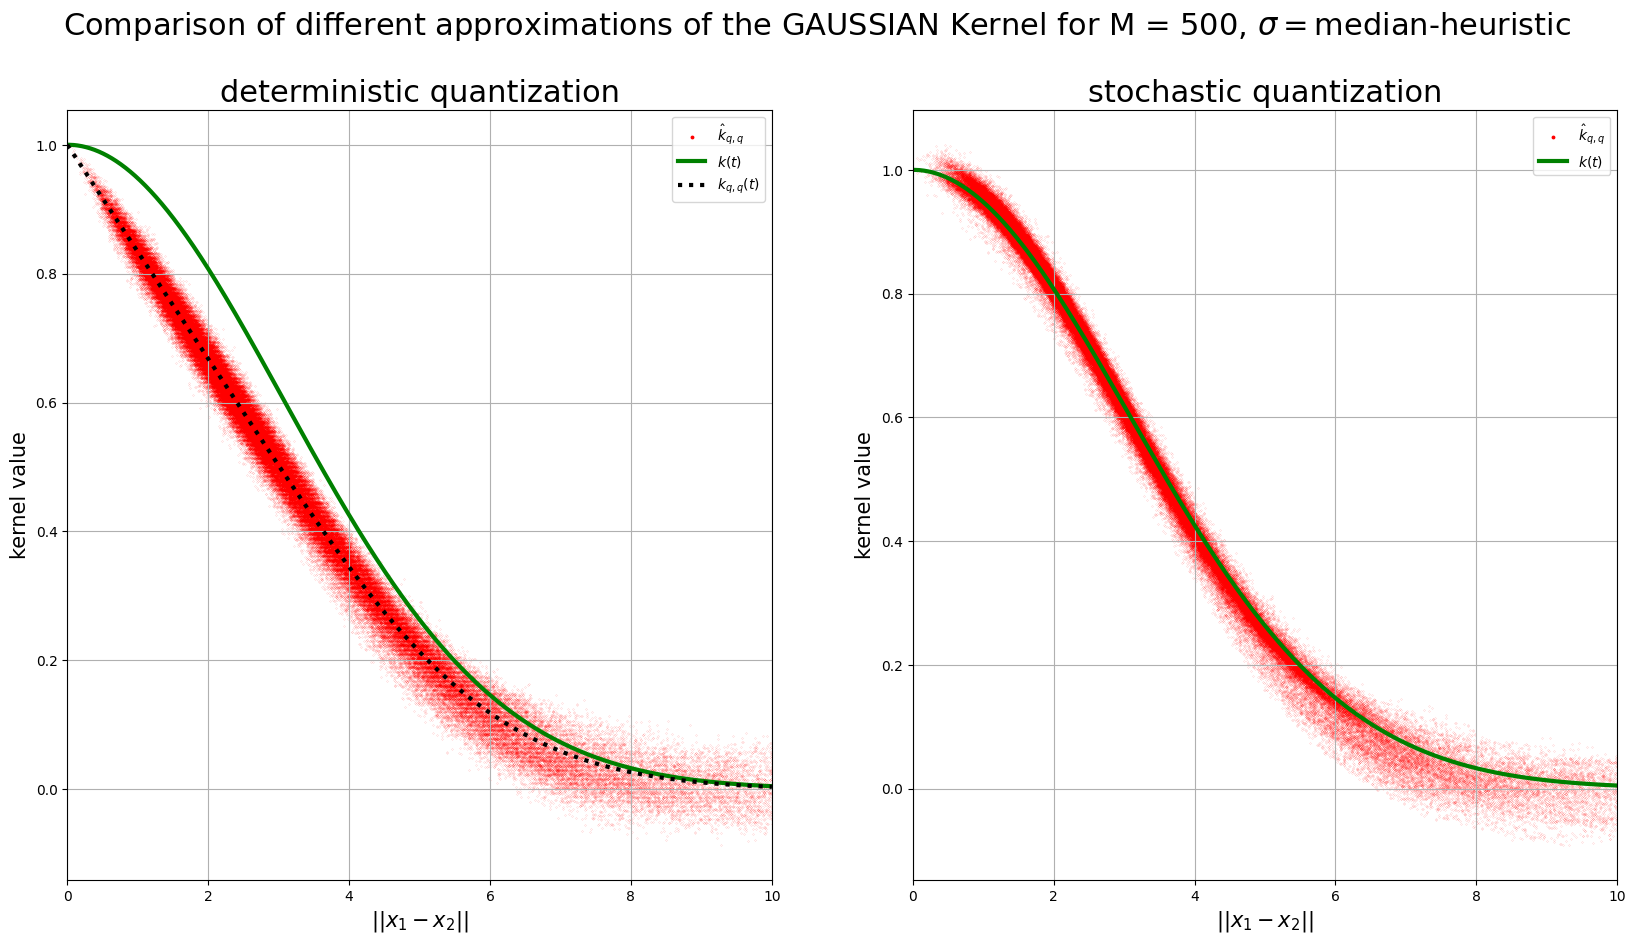
\includegraphics[width=1\textwidth]{pics/comparison_diff_approx_gaussian.png}
        \caption{Comparison of different approximations of the Gaussian Kernel for $M = 500$, $\sigma=$ median-heuristic on the CASP dataset}
        \label{fig:gaussian_kernel_comparison}
    \end{figure}

    \textbf{TBA comparison in learnign procedures + teoretical justification of everything}


    \begin{figure}[htbp]
        \centering
        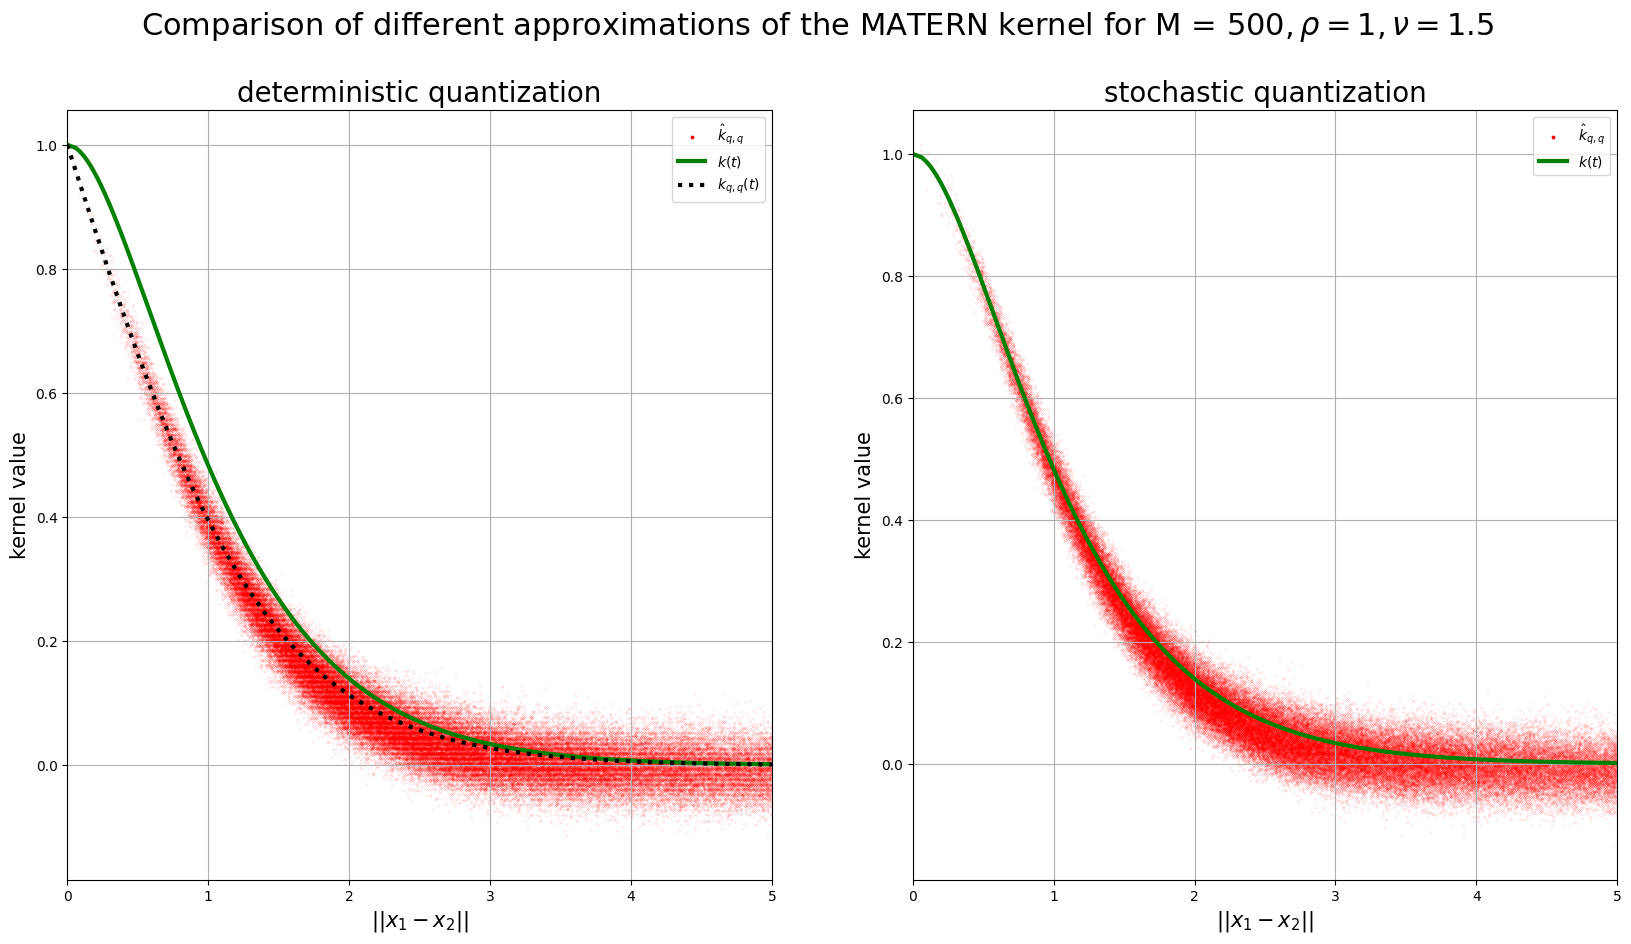
\includegraphics[width=1\textwidth]{pics/comparison_diff_approx_matern.png}
        \caption{Comparison of different approximations of the Matern Kernel for $M = 500$, $\rho = 1$, $\nu = 1/2$ on the CASP dataset}
        \label{fig:matern_kernel_comparison}
    \end{figure}


    \begin{figure}[htbp]
        \centering
        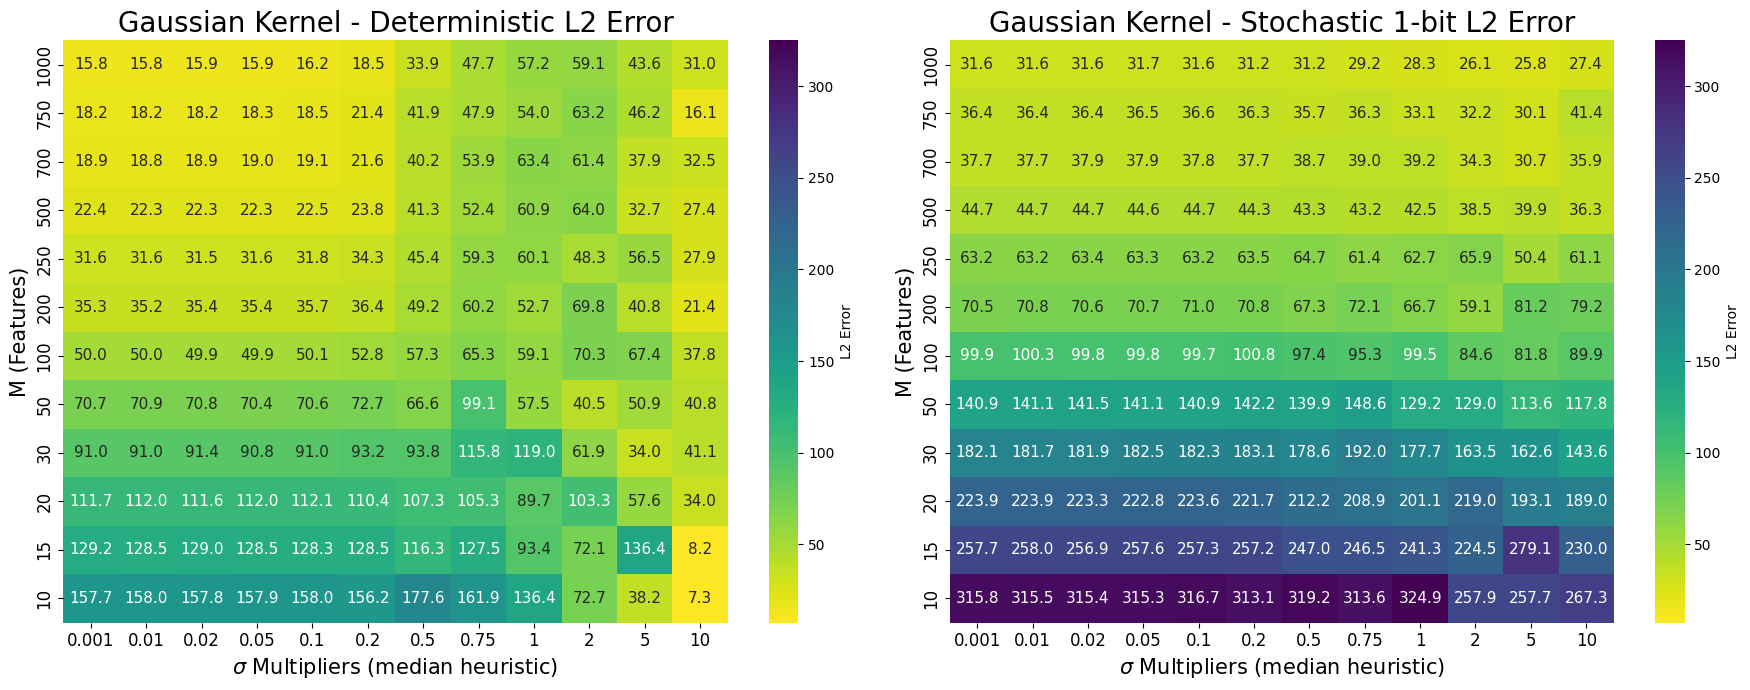
\includegraphics[width=1\textwidth]{pics/Gaussian_Kernel_htm_comparison.png}
        \caption{Heatmap of the $L^2$ error for different bandwidths $\sigma$ and number of random features $M$ on the CASP dataset}
        \label{fig:gaussian_kernel_htm_comparison}
    \end{figure}

    \begin{figure}[htbp]
        \centering
        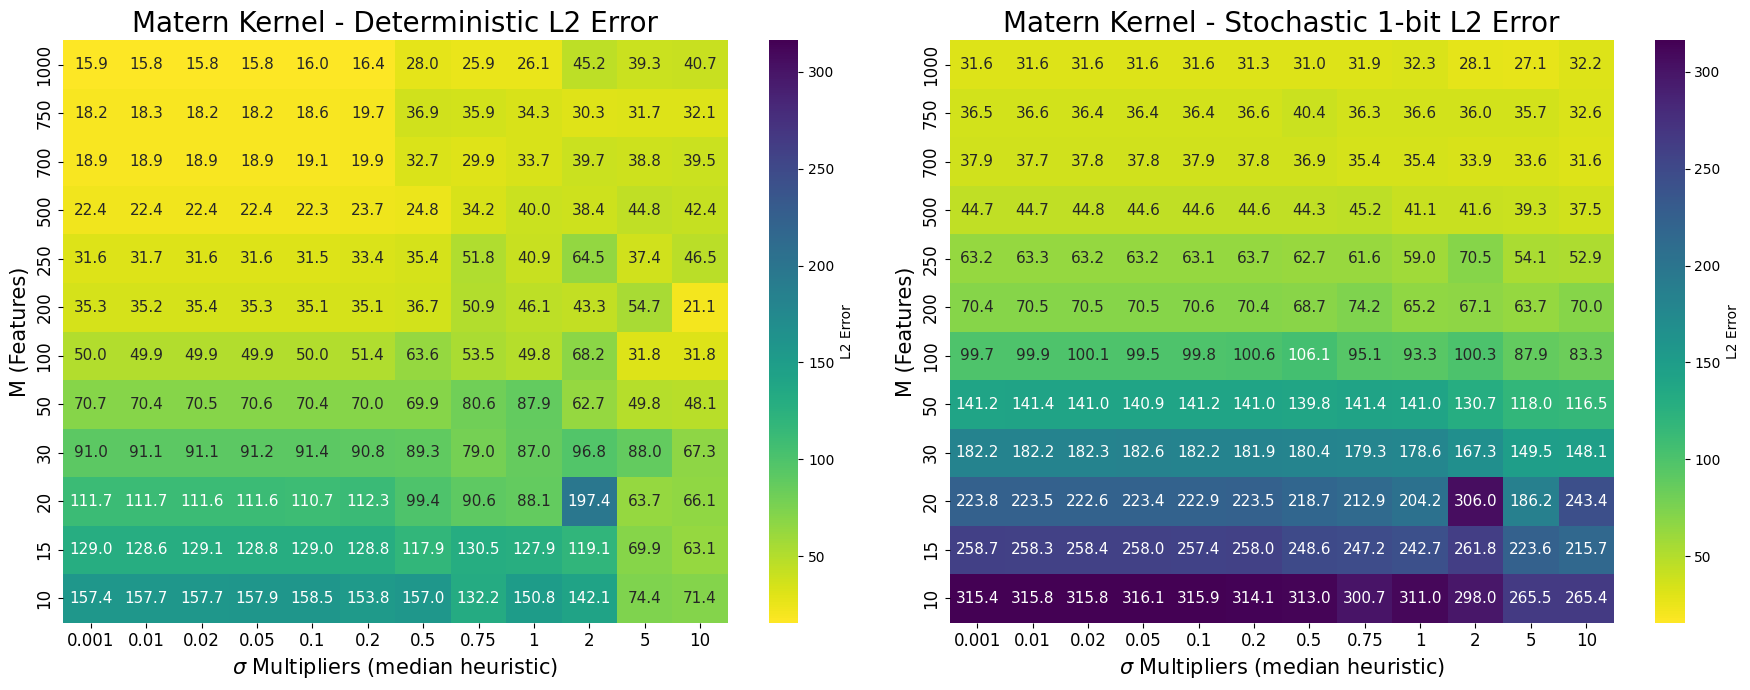
\includegraphics[width=1\textwidth]{pics/Matern_Kernel_htm_comparison.png}
        \caption{Heatmap of the $L^2$ error for different smoothness parameters $\nu$ and fixed $\rho=1$ on the CASP dataset}
        \label{fig:matern_kernel_htm_comparison}
    \end{figure}













\end{chapter}